%!TEX root = thesis.tex
\chapter{Theory}

To encompass all theory regarding stellar structure, evolution, and their
atmosphere is far beyond the scope of this thesis. Rather the theory needed is
presented below with highlights on the most important aspects.

\section{Stellar structure}

The structure of a non-rotating spherical stars can be described by five rather
simple differential equations \citep[see e.g.][]{kippenhahn} presented below:
\begin{enumerate}
    \item \textbf{Equation of Continuity}
        \nicebreak
        Relation between the mass, $m$, the density, $\rho$, at a symmetric
        shell at radius $r$
        \begin{align}
            \Aboxed{\pd{r}{m} &= \frac{1}{4\pi r^2\rho}.}
        \end{align}

    \item \textbf{Equation of Hydrostatic Equilibrium}
        \nicebreak
        The equation of hydrostatic equilibrium shows how a star in equilibrium
        is balanced between two forces. The inward force from gravity and the
        outward force from pressure, $P$,
        \begin{align}
            \Aboxed{\pd{P}{m} &= -\frac{Gm}{4\pi r^4}.}
        \end{align}
        When working with asteroseismology a time dependent perturbation to this
        equation is added \citep[see e.g.][for a thorough discussion]{Aerts2010}.
        However, this term is neglected here.


    \item \textbf{Equation of Energy Conservation}
        \nicebreak
        The equation of energy conservation shows how the energy is produced and
        lost throughout the star.
        \begin{align}
            \Aboxed{\pd{l}{m} = \epsilon - \epsilon_\nu + \epsilon_g,}
        \end{align}
        where $\epsilon$ is the energy production in the centre of the star,
        $\epsilon_\nu$ is the energy lost by neutrinos which is always
        positive, $\epsilon_g$ is a source function of time-dependent terms,
        and $l$ is the luminosity at $m$. $\epsilon_g$ comes from the fact that
        non-stationary shells can change its internal energy, and thus exchange
        mechanical energy with neighbouring shells.

    \item \textbf{Equation of Energy Transport}
        \nicebreak
        Energy transportation throughout the star is described with the
        following equation
        \begin{align}
            \Aboxed{\pd{T}{m} &= -\frac{GmT}{4\pi r^4P}\nabla_\tm{rad},}
        \end{align}
        where $\nabla_\tm{rad}$ is the radiative temperature gradient, and $T$
        is the temperature. The value of the temperature gradient compared to
        the radiative temperature gradient tells if the energy is transported by
        convection or radiation. In our Sun the outer layer are convective while
        the inner layer are radiative.

    \item \textbf{Equation of Chemical Composition}
        \nicebreak
        In this last equation we see the evolution of an element, $X_i$, when
        it reacts with other elements with reaction rates $r_{ji}$ and $r_{ik}$
        \begin{align}
            \Aboxed{\pd{X_i}{t} &= \frac{m_i}{\rho} \Bigl( \sum_j r_{ji} - \sum_k r_{ik}\Bigr).}
        \end{align}
        Note that this is the only time-dependent equation of the five
        presented.
\end{enumerate}

These five fundamental equations are implemented in stellar evolutionary codes,
which we will use in later chapters. The many different codes that exist take
other things into account, e.g the star can rotate, and it may not always be in
hydrostatic equilibrium (this is important if we want our star to pulsate). For
simplicity we have only presented time-dependence in the Equation of Chemical
Composition since timescales of rotation, pulsations, and activity are much
shorter than the long timescale found in chemical composition changes.


\section{Stellar atmosphere}

Much of this Section is inspired by \citet{Gray2006}. While all the figures here
were made by the author of this thesis, most of them can be found in
\citet{Gray2006} as well.

Stellar atmospheres are rather complicated. This is where the light produced in
the interior of the stars are released. However, the atmosphere of a star is not
transparent to all light, and some of the light is absorbed in the atmosphere
and later emitted in a random direction. The different elements in the
atmosphere is the reason for absorbing light at specific wavelength. The
strength of the absorption depends on the physical conditions in the atmosphere,
the effective temperature ($T_\mathrm{eff}$), the pressure/gravity ($\log g$),
the overall metallicity ($[\ion{Fe}/\ion{H}]$), the specific abundance of a
given element if different from the overall metallicity ($A$), and the atomic
characteristics of the transition coursing the absorption line.

It is important to know the fraction of atoms excited to the $n$th energy level,
$N_n$. This fraction is proportional to the statistical weight $g_n$ and the
Boltzmann factor and is described as:
\begin{align}
    \Aboxed{ \frac{N_n}{N} = \frac{g_n}{u(T)} 10^{-\theta\chi_n}} \tag*{Boltzmann}
\end{align}
This equation is also called the Boltzmann equation. Here $N$ is the total
number of atoms per unit volume, $u(T)=\Sigma g_i e^{-\chi_i/kT}$ is the
partition function, $k$ is Boltzmann's constant, $T$ is the temperature, and
$\chi_n$ is the excitation potential for the lower energy level.

While atoms can get excited following Boltzmann's equation above, they can also
get ionized. The ionization ratio for a collision dominated gas (which is a good
approximation for FGKM stars) is described by the Saha equation. This equation
relate the ratio of atoms in state $r$ to atoms in the excited state above for
the same element, $r+1$, in the following way:
\begin{align}
  \Aboxed{ \frac{N_{r+1}}{N_r} = \frac{1}{P_e} \frac{(2\pi m_e)^{3/2}(kT)^{5/2}}{h^3} \frac{2u_{r+1}(T)}{u_r(T)} e^{-I/kT} = \frac{\Phi(T)}{P_e}} \tag*{Saha}
\end{align}
here $m_e$ is the electron mass, $h$ is Planck's constant, $I$ is the ionization
potential of the neutral atom, and $\Phi(T)$ is all not related to the electron
pressure, $P_e$.

The atomic lines are characterised by few quantum mechanical descriptors.
\begin{itemize}
  \item The wavelength describes between which energy levels there is a
        transition, i.e. at which wavelength the light is absorbed.
  \item The ionization state, i.e. is it a atom element absorbing or a ionized
        atom.
  \item The excitation potential. This gives an idea how deep in the atmosphere
        a line is formed. If $\chi$ is high, then higher temperatures (i.e.
        higher random motion and more collisions between the atoms) is required
        for forming the absorption line. These higher temperatures are found
        deeper in the atmosphere.
  \item The oscillator strength, $\log \mathit{gf}$, is related to the atomic
        transition probability.
  \item The damping coefficients, is a natural damping (also known as radiation
        damping) caused by the uncertainty of lifetime in an energy level
        according to Heisenberg's uncertainty principle. This is related to a
        uncertainty in the energy level and thus a natural broadening is
        introduced.
\end{itemize}
These are essential to know from either theoretical calculations or experiments.
The oscillator strength is a quantity that is difficult to measure, and this
is often changed when absorption lines are matched with real observations of
e.g. the Sun. This is a way of calibrating a line list and will be described in
detail in \sref{sec:linelist}.

It is important to mention that one of the main differences between absorption
lines in optical and near-infrared is the excitation potential. The energy
levels of an atom gets denser packed as the energy level increase as shown in
\fref{fig:elevel} for hydrogen. For hydrogen the energy levels $E_n$ follow the
very simple formula from Bohr's atomic model, $E_n=\frac{\SI{-13.6}{eV}}{n^2}$,
where $n$ is the principal quantum number, and \SI{13.6}{eV} is the ionization
energy for hydrogen, i.e. the minimum amount of energy required to ionize
hydrogen. The energy levels for heavier atoms show a similar structure. The
outer electron for a multi-electron atom is partially shielded from the nucleus
by the inner electrons, and thus does not experience the full charge $Z$ but
rather an effective charge $Z_\mathrm{eff}$, giving the expression
\begin{align}
  E_n = -hcR_\infty\frac{Z_\mathrm{eff}^2}{n^2},
\end{align}
where $h$ is Planck's constant, $c$ is the speed of light, and $R_\infty$ is
Rydberg's constant.

With increasing $n$ the energy levels get closer, or in other words the photon
required to excite an electron from one energy level to a neighbouring state
will get redder. These redder photons used for exciting an atom are the
absorption lines seen in the NIR. However, the excitation to the lower state is
from thermal motion and not coursed by photons. Since tight energy levels
require a highly excited lower state, the temperature required here are similar
high, which means that the NIR lines are typically formed in the deeper layers
of the atmosphere compared to absorption lines seen in the optical part of the
spectrum.

\begin{figure}[htpb!]
    \centering
    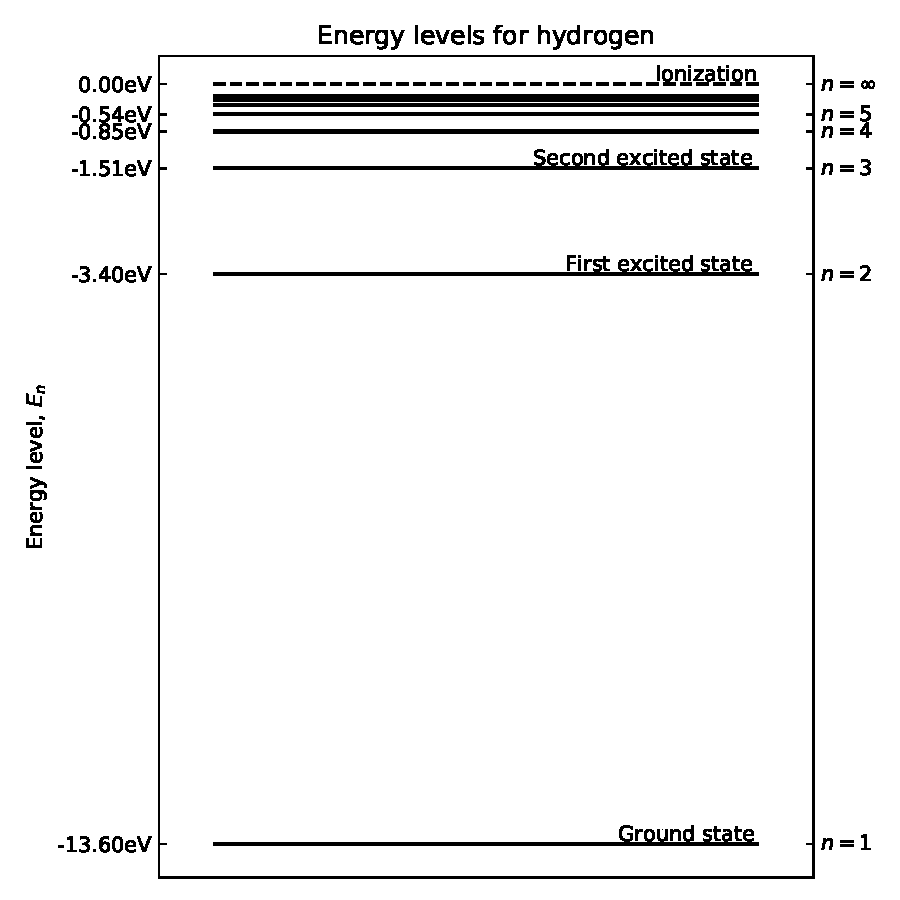
\includegraphics[width=1.0\linewidth]{figures/energyLevels.pdf}
    \caption{Energy levels for hydrogen, $E_n=\frac{\SI{-13.6}{eV}}{n^2}$.}
    \label{fig:elevel}
\end{figure}

The above discussed energy transitions are purely electronic, however there
exists so called fine structure transitions as well. This is due to the spin of
the electron (or magnetic moment) interacting with the orbital angular momentum
of the electron. This leads to a splitting of the absorption line. In atoms
there also exists an even finer structure, commonly known as the hyperfine
structure. This structure arise due to the interaction between the magnetic
field created by the electrons and the nuclear spin. These splittings are
important to consider for some transitions and some atoms. For \ion{Fe}{} the
hyperfine structure is not important since the net nuclear spin (of protons) is
0 because there is an even number, hence hyperfine structure is only important
for atoms with an odd number of protons. There are other splitting and shift for
spectral absorption lines like the Zeeman splitting coursed by an external
magnetic field, and the Stark effect splitting a line due to an external
electric field. These two last effect are minor and will not be discussed more,
however it is worth noting that the Zeeman splitting can be used to measure the
strength of a magnetic field in a star if this is strong enough.



\subsection{Atmosphere models}
\label{sec:atmospheremodels}

In order to derive abundances or calculate a synthetic spectrum, two main things
are needed: 1) And atmosphere model, and 2) a radiative transfer code that
solves the equations above. There are different atmosphere models available.
Throughout this thesis the ATLAS9 model atmosphere are used by
\citet{Kurucz1993}. Other mention-able atmosphere models includes MARCS models
\citep{Gustafson2008} and the PHOENIX models \citep{Husser2013}. An atmosphere
model is a file with typically 72 layers. Each layer includes physical
quantities such as temperature, gas and electron pressure, the optical depth,
etc. The models can be calculated on the fly, but it is common practise to
pre-calculate a grid of atmosphere models at certain $T_\mathrm{eff}$, $\log g$,
and $[\ion{Fe}/\ion{H}]$. A specific atmosphere model is then obtained from this
grid by interpolating from nearest neighbours. The interpolation code used
throughout this work includes the four nearest neighbours in the
$T_\mathrm{eff}$-space, and the two nearest neighbours in both the $\log g$- and
$[\ion{Fe}/\ion{H}]$-space, in total $4\times2\times2=16$ atmosphere models to
generate a single interpolated atmosphere model.



\subsection{Radiative transfer code - \MOOG}

As mentioned above, a radiative transfer code is needed to solve the equations
above. There are many different codes that does this. Here the \MOOG code us
used \citep{Sneden1973}. This code has different drivers, only some are used
here.

\begin{itemize}
  \item Derive a theoretical equivalent width (see \sref{sec:EW} for details)
        for a given star, i.e. atmosphere model with a given set of atmospheric
        parameters.
  \item Derive line abundance from a measured equivalent width for a given model
        atmosphere.
  \item Calculate a synthetic spectrum for a given model atmosphere and atomic
        line list.
  \item Calculate the curve-of-growth for an atomic line.
\end{itemize}
There exists other drivers as well, but these are the ones used here. Some only
for visualising the figures below.



\subsection{The equivalent width}
\label{sec:EW}

Measuring the equivalent width (EW) of spectral lines are important for some
analysis of stellar spectra. The EW is a measure of the strength of the line,
and dependent on the atmospheric conditions in where the spectral line is
formed, such as $T_\mathrm{eff}$, $\log g$, $[\ion{Fe}/\ion{H}]$, and
$\xi_\mathrm{micro}$.

\begin{figure}[htpb!]
    \centering
    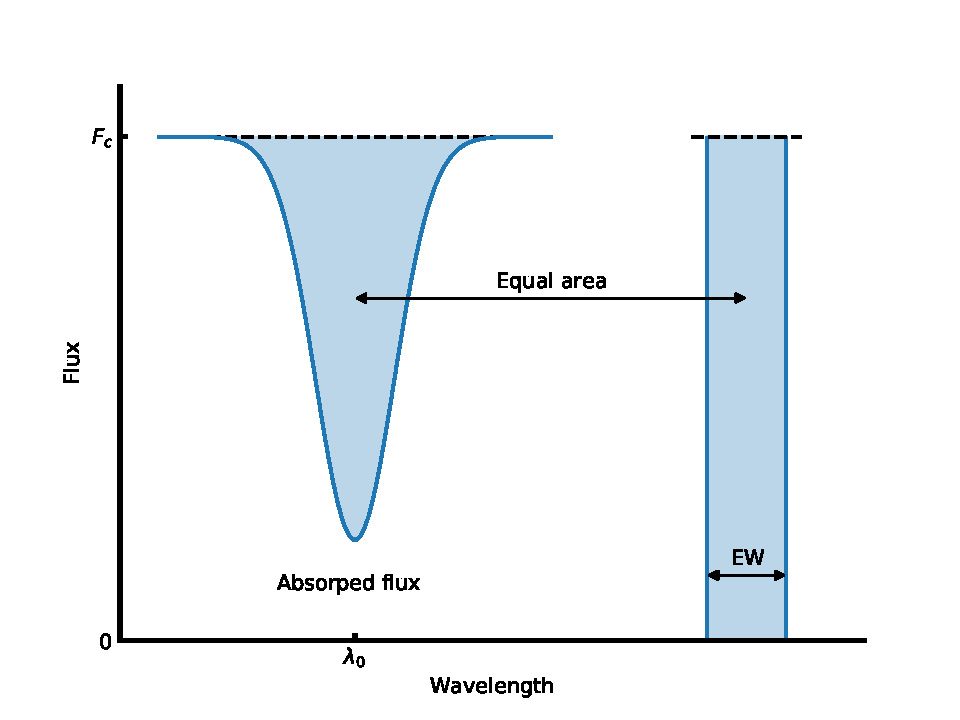
\includegraphics[width=1.0\linewidth]{figures/ewTheoretical.pdf}
    \caption{An absorption line centred at $\lambda_0$ normalised at the flux
             level $F_c$. The area of the absorption line to the left is equal
             to the blue shaded area in the rectangle to the right with width
             EW.}
    \label{fig:ewTheoretical}
\end{figure}

The EW is mathematically described as integrating over the entire line, and
assign this area to a rectangle from 0 to the continuum flux ($F_c$) with the
width, EW. This is illustrated in \fref{fig:ewTheoretical} and the equation
below: \begin{align} EW = \int_{0}^{\infty} \frac{F_c-F(\lambda)}{F_c} d\lambda,
\end{align} where $\lambda$ is the wavelength. This is integral is assuming
there is only one single line, hence the integral is over all wavelength. In
practice the integral is calculated in small windows around a spectral line. See
\sref{sec:measureEW} for more details on how this is performed in practice. The
unit of the EW is the same as the wavelength used. Throughout this thesis we
will use \AA{}ngstr\"{o}m (1\AA$=\SI{0.1}{nm}$) for the wavelength, and m\AA{}
for the EW.


\subsubsection{Temperature dependence}

As mentioned above the EW depends on the atmospheric parameters. The dependence
on $T_\mathrm{eff}$ is the strongest dependence. At low $T_\mathrm{eff}$ neutral
elements, say \ion{Fe}{I}, are the strongest lines as the number of ionized
atoms are too small to contribute significantly to the EW. This is the result
the Saha equation. As $T_\mathrm{eff}$ increases \ion{Fe}{I} is converted into
ionized \ion{Fe}{II}. Slowly, as the number of \ion{Fe}{I} decreases so does the
EW, and likewise as the number of \ion{Fe}{II} increases so does the EW. This
goes on until second ionized atoms, \ion{Fe}{III}, are formed and the same
situation arise again. This is illustrated in \fref{fig:ewTeff} where the EW of
two iron lines, one neutral and one ionized, are plotted against
$T_\mathrm{eff}$. These two lines have similar EW in the Sun:
$\SI{46.2}{m}$\AA{} and $\SI{53.9}{m}$\AA{} for the \ion{Fe}{I} and \ion{Fe}{II}
line respectively.

\begin{figure}[htpb!]
    \centering
    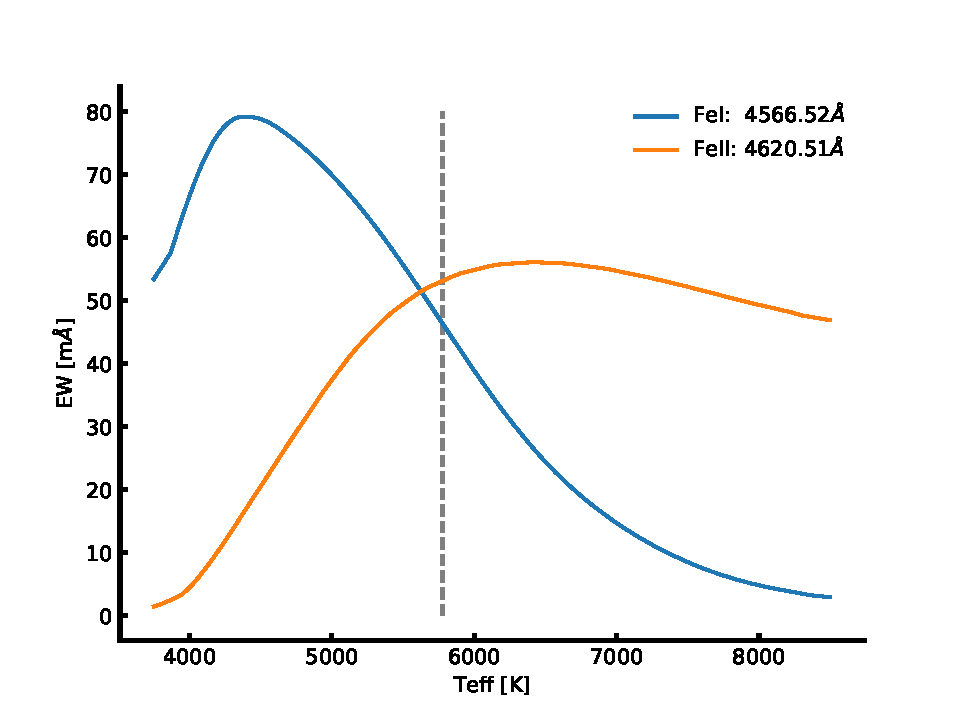
\includegraphics[width=1.0\linewidth]{figures/ewTeff.pdf}
    \caption{The EW for a \ion{Fe}{I} and \ion{Fe}{II} line with increasing
             $T_\mathrm{eff}$. The two lines have similar EW in the Sun and are
             found in the optical part of the spectrum. The vertical line show
             the solar $T_\mathrm{eff}$.}
    \label{fig:ewTeff}
\end{figure}


\subsubsection{Pressure dependence}

Pressure dependence in the stellar atmosphere can be related to the gravity
dependence. There are many ways to measure the pressure, and thus the gravity
which is what is ultimately the goal with the measurement of $\log g$. Below are
listed some of the most common methods to measure $\log g$ from spectroscopy.

\begin{itemize}
  \item Continuum: The Balmer jump is the only continuum feature sensitive
        enough to estimate the $\log g$.
  \item Hydrogen lines: Hydrogen profiles are pressure sensitive and can
        therefore be used to estimate $\log g$. However, the gravity dependence
        rapidly diminishes for temperatures above $\SI{10\,000}{K}$.
  \item Other strong lines: There exists other strong lines with
        pressure-broadened wings such as the \ion{Ca}{II} H and K lines. These
        are better for cooler stars than the hydrogen lines described above.
  \item Weak lines: By comparing two stages of ionization for the same element
        it is possible to obtain $\log g$ using weaker or modestly strong lines.
\end{itemize}
In this thesis weak lines are used to measure $\log g$. More specifically a
comparison between \ion{Fe}{I} and \ion{Fe}{II} lines are used. For FGK stars,
as the atmosphere contracts (i.e. $\log g$ increases) the pressure likewise
increases, which in turn means that both the gas pressure, $P_g$, and electron
pressure, $P_e$, increases. Since hydrogen is the main electron contributor, but
not fully ionized for these stars, the electron pressure is much smaller that
the gas pressure. The gas pressure follow a simply empirical approximation with
gravity:
\begin{align}
  P_g \approx \mathrm{constant}\, g^{2/3},
\end{align}
where $g$ is the gravity. The electron pressure is given by
\begin{align}
  P_e \approx \mathrm{constant}\, g^{1/3}.
\end{align}

There are three cases for which a line show dependence on gravity, when
considering only weak lines:
\begin{enumerate}
  \item A weak line formed by any ion or atom, where most of the element is in
        the next higher ionized state.
  \item A weak line formed by any ion or atom, where most of the element is in
        the same ionized state.
  \item A weak line formed by any ion, where most of the element is in the next
        lower ionized state.
\end{enumerate}

Using the Saha equation for case 1, it is important to note that the number of
the atoms in the highest state is roughly equal to the total number of atoms of
that element, $N_{r+1}\approx N$. Hence
\begin{align}
  N_r \approx \mathrm{constant}\,\, P_e
\end{align}
which means that the line absorption coefficient is
\begin{align}
  l_\nu \approx \mathrm{constant}\,\, N_r \approx \mathrm{constant}\,\, P_e.
\end{align}
The strength of a weak line, $R$, is proportional to the ratio of the line to
the continuous absorption coefficient, $\kappa_\nu$
\begin{align}
  R = \frac{F_c-F_\lambda}{F_c} = \mathrm{constant}\,\, \frac{l_\nu}{\kappa_\nu}.
\end{align}
When negative hydrogen dominates $\kappa_\nu$ which is the case here it is
proportional to the electron pressure, $\kappa_\nu\propto P_e$ which means the
line strength is not proportional to to electron pressure:
\begin{align}
  R = \frac{l_\nu}{\kappa_\nu} \approx \mathrm{constant}.
\end{align}

For case 2, the approach is the same, here
$N_r\approx N_{r+1}\approx N= \mathrm{constant}$. This leads to
$l_\nu\approx\mathrm{constant}$, eventually giving
\begin{align}
  R=\frac{l_\nu}{\kappa_\nu} \approx \frac{\mathrm{constant}}{P_e} \approx \mathrm{constant}\,\, g^{-1/3}.
\end{align}
Only the first two cases are relevant for solar-type stars used in this thesis,
and the relation for the third case will be omitted.

In \fref{fig:ewGravity} is shown how the \ion{Fe}{II} line used previously
change with $\log g$. The curve of growth is shown in the upper panel, while a
synthetic spectrum for each $\log g$ is presented in the lower left panel. It is
clear that the ionized line is sensitive to $\log g$ as shown in the lower right
panel, where the correlation between the abundance and $\log g$ is 0.40. This is
expected as can be seen in \citet[][Table 16.1]{Gray2006}. There is used
$\delta\log A/\delta\log g$ as an indicator, and for neutral elements the
correlation is much weaker. It is important to note that the correlation does
change with $T_\mathrm{eff}$ and the element used.

\begin{figure}[htpb!]
    \centering
    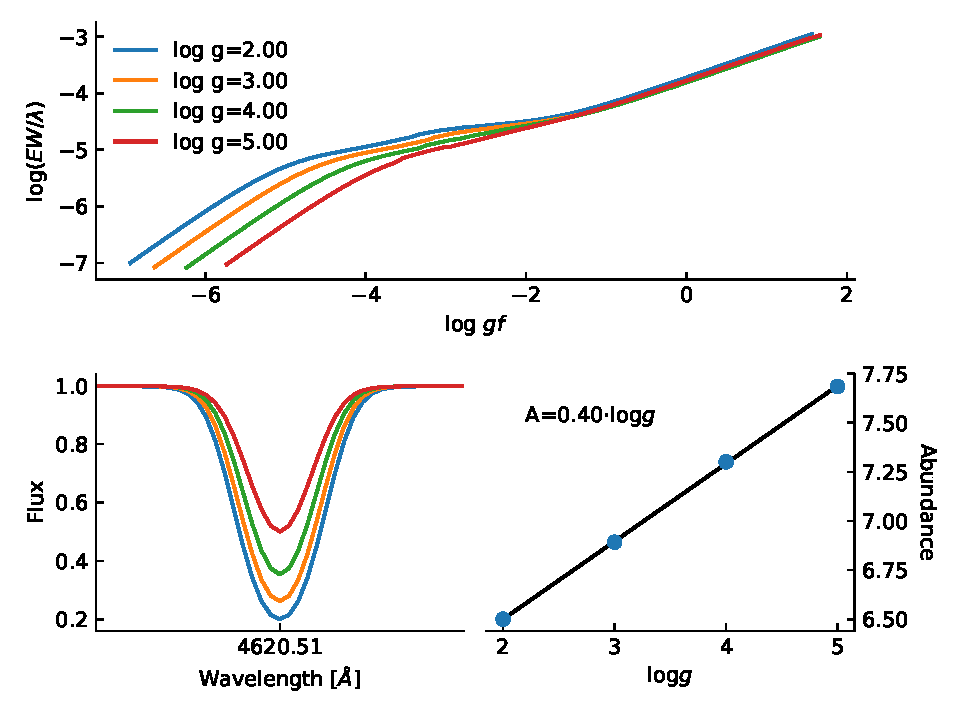
\includegraphics[width=1.0\linewidth]{figures/ewGravity.pdf}
    \caption{\emph{Upper panel}: Curve of growth for same \ion{Fe}{II} used in
             \fref{fig:ewTeff} for four different $\log g$ values. Here it is
             the weak lines mostly affected by the change in $\log g$.
             \emph{Lower left panel}: Synthetic spectra of the same line. The
             colour scale is the same.
             \emph{Lower right}: The abundance for the line at different
             $\log g$. A strong correlation (0.40) is seen.}
    \label{fig:ewGravity}
\end{figure}




\subsubsection{Abundance dependence}

The abundance of a given element obviously has an effect on the EW. The more
abundant an element is, the more photons can be absorbed thus increasing the EW.
However, the relationship is not strictly linear. For weak lines (GIVE RANGE) EW
is approximately linear with the abundance, however it reach a plateau where the
core of the line saturates. In this regime the EW only increases slowly, until
the absorption "spills" into the wings and the increase is again linear.
However, for these strong lines the profile is no longer Gaussian. The curve of
growth for the same \ion{Fe}{I} line used in \fref{fig:ewTeff} is shown in
\fref{fig:cog}. Instead of EW it is common to use the reduced EW, $\log
(EW/\lambda)$\footnote{The reduced EW is useful since it normalises
Doppler-dependent phenomena, such as microturbulence and thermal broadening.},
which we will use more later. Instead of the abundance of a line, the oscillator
strength, $\log \mathit{gf}$, is used.

\begin{figure}[htpb!]
    \centering
    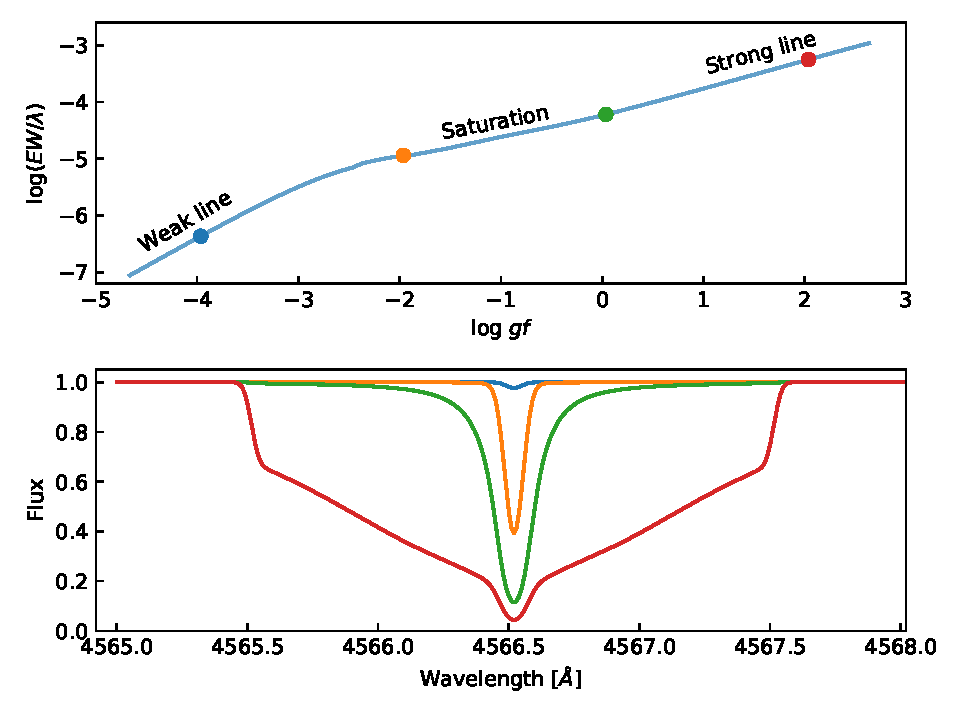
\includegraphics[width=1.0\linewidth]{figures/cog.pdf}
    \caption{\emph{Upper panel:} Curve of growth of the same \ion{Fe}{I} line as
             used in \fref{fig:ewTeff}. Four points are marked which is shown in
             the \emph{lower panel} as a synthetic spectral line. The RW (proxy
             for EW) is clearly increasing with $\log \mathit{gf}$ (proxy for
             abundance).}
    \label{fig:cog}
\end{figure}


\subsubsection{Microturbulence}

Small-scale motion, that is motion of material at length scales small compared
to the unit optical depth, are called microturbulence, $\xi_\mathrm{micro}$.
This is not to be confused with macroturbulence, which is motion of material at
scales larger than the unit optical depth. The latter is associated with
granulation and will not be discussed further in this thesis.
$\xi_\mathrm{micro}$ comes into play when looking at the curve of growth for
saturated lines (i.e. between green and red points in \fref{fig:cog}). If no
$\xi_\mathrm{micro}$ is assumed, then the measured abundance is higher than
predicted by models based on thermal and damping broadening alone. In
\fref{fig:cog_vt} is shown three curves of growth with
$\xi_\mathrm{micro}={\SI{0.5}{km/s}, \SI{2.5}{km/s}, \SI{5.0}{km/s}}$. As
$\xi_\mathrm{micro}$ increases, so does the EW and hence the abundance.

\begin{figure}[htpb!]
    \centering
    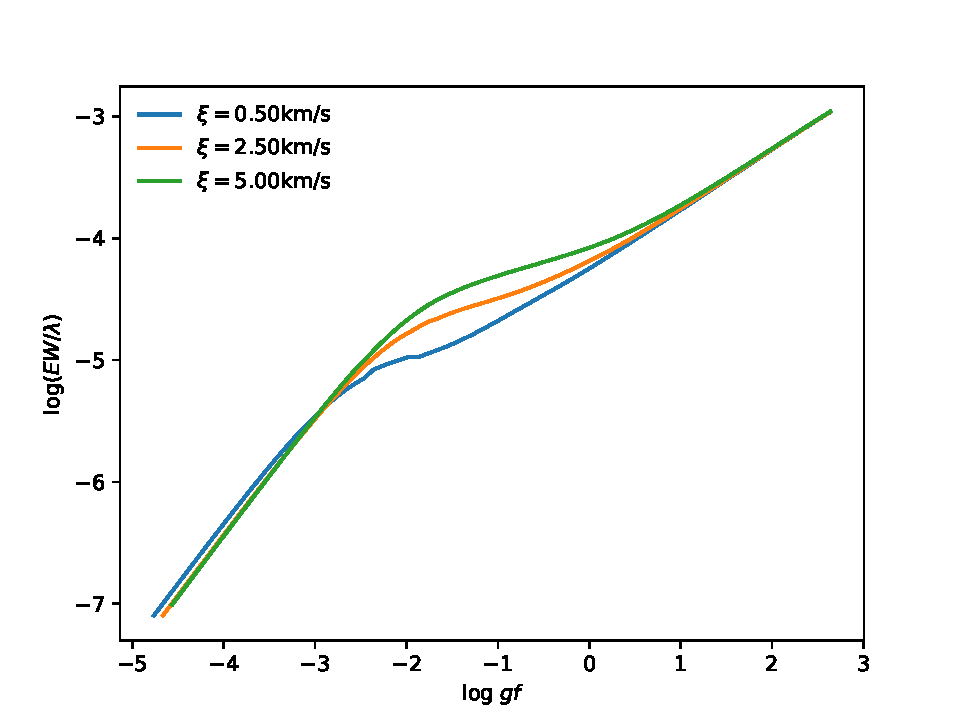
\includegraphics[width=1.0\linewidth]{figures/cog_vt.pdf}
    \caption{Curve of growth for three different values of $\xi_\mathrm{micro}$.
             The EW is increasing with increasing $\xi_\mathrm{micro}$.}
    \label{fig:cog_vt}
\end{figure}

The broadening of an absorption line measured by the shift in wavelength,
$\Delta\lambda$, when $\xi_\mathrm{micro}$ is included is defined as:
\begin{align}
  \Delta\lambda = \frac{\lambda_0}{c} \sqrt{\frac{2kT}{m} + \xi_\mathrm{micro}^2},
\end{align}
where $c$ is the speed of light, $\lambda_0$ is the rest wavelength of the given
line, $k$ is Boltzmann's constant, $T$ is the temperature, and $m$ is the mass
of the atom. Setting $\xi_\mathrm{micro}=\SI{0}{km/s}$, we end up with thermal
broadening.


\section{Line list and atomic data}
\label{sec:linelist}

As mentioned above, the atomic data of the absorption lines are required. These
data can be found in a database such as \emph{The Vienna Atomic Line Data Base}
(VALD) \citep{VALD1,VALD2}. For compiling a usable iron line list, all
theoretical transitions in a given wavelength range are requested from VALD. In
the near-infrared (NIR), YJHK bands, there are several thousands of theoretical
transitions. The EWs are measured (see \sref{sec:measureEW}) for all these
lines using a solar spectrum \citep[][is used here]{Hinkle1995}. Here there are
four possible outcomes. 1) A line can not be measured and is thus discarded, 2)
the EW of the line is weak (below 5 m\AA{}) to be reliable, 3) the EW of the
line is too strong ( above 150 m\AA{}) and the line show non-linear behaviour in
the curve-of-growth (see \fref{fig:cog}), or 4) the EW of the line is between
the two limits and is then added to the final line list.

After removing lines which EW is outside the range of EW mentioned above, it is
good practise to have a visual inspection. Here one should look for severe line
blending with other absorption lines which might prove problematic and
unreliable measurements of the EW. If the reference spectrum used, here for the
Sun, is not corrected for telluric lines, it is also a good idea to remove lines
which exists amidst forest of telluric lines, as these absorption lines might
fall on the telluric lines, if the star observed has a different radial velocity
(RV).

When blended lines and otherwise lines which shows strange features (can be in a
forest of telluric lines), the last step is to calibrate the atomic data. As
mentioned above, this is done by changing the $\log \mathit{gf}$ value for a
given line, until it has the desired determined abundance. In this case, an iron
line should have the abundance of 7.47 using the values from
\citet{Gonzalez2000}, when using a solar atmosphere model. There is a simple
anti-correlation between the determined abundance from the measured EW and the
$\log \mathit{gf}$, so a simple bisector minimization can be used to find the
best $\log \mathit{gf}$. It is important to calibrate the $\log \mathit{gf}$
when changing the version of \MOOG (or if other radiative transfer codes are
used), the atmosphere model and version of those, and even the interpolation of
the atmosphere models. These changes in $\log \mathit{gf}$ should be minor
compared to the change from the VALD database and those we arrive at when
calibrated for the Sun.



\section{Spectrographs}
\label{sec:spectrographs}

This chapter will be focused on some of the available spectrographs for deriving
stellar atmospheric parameters using the method described in
\sref{sec:parameters}. For this we need a spectrum of both high resolution and
high signal-to-noise ratio, S/N, which combined will be called a high quality
spectrum. In order to get reliable results, a spectral resolution of at least
$R=\frac{\lambda}{\Delta\lambda}=25\,000$ is needed. A $S/N\approx 100$ is at
least needed to obtain the parameters. These are approximately values since it
can vary across different spectral classes, e.g. it is often relatively easy to
obtain parameters of a solar-twin while it gets increasingly difficult as
especially $T_\mathrm{eff}$ diverges in either direction from the solar value.
Naturally the higher quality the spectrum is (both resolution and S/N), the
better the results will be obtained. It is common practise to increase the S/N
for a spectrum by co-adding a sample of lower S/N spectra of the same star from
the same spectrograph. This is often used if the star of interest is so dim that
it takes several observations to reach a sufficient high S/N. Another case is
when spectra have been obtained from the archive. The scientific goal can be
very different, e.g. obtaining radial velocities (RV) where a much lower S/N is
needed, however here numerous spectra are needed. It is common to search for
exoplanets with the RV detection method, where multiple spectra are obtained,
and the stellar parameters are then obtained after co-adding the multiple
spectra. It is of course important to put the spectra on a common RV, usually at
\SI{0}{km/s}.

Spectrographs work in different wavelength regions. The most used region is the
optical part of the spectrum, which is also ideal for studying FGK stars with
relative low line blending and low telluric contamination. In the recent years
there has been an increase of NIR spectrographs. These will mainly be used to
study the distant Universe, i.e. at high red-shifts, and cool objects in our own
galaxy. Especially interesting are the M stars which consist of around 70\% of
all stars in our galaxy \citep{Bochanski2010}. These stars are intrinsic dim
because of their low $T_\mathrm{eff}$, ranging from \SIrange{2200}{3500}{K},
hence most of their light emitted will be in the NIR. It is advantageous to
collect as much light as possible from these dim stars, since reaching a similar
S/N in the optical would be more time expensive. The cool M stars have more
molecules in the atmosphere than their hotter counterparts. This can be seen in
the spectrum, where molecular lines greatly depress the continuum (and
me\change{Remove stupid joke!}), making EW measurements difficult. This
continuum depression is much larger in the optical than the NIR, giving another
motivation for studying stars in this wavelength region.
